\setcounter{step}{0}
%------------------------------------------
% information doc
\subsection{Tapenarde}
\PrepTime{10}
\CookingTime{0}
\CookingTempe{0}
\TypeCooking{Mixovanie}
\NbPerson{4}
\Image{0 0 430 430}{images/florentin} %style 2
%------------------------------------------

\begin{ingredient}
%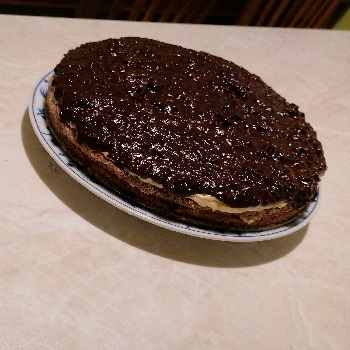
\includegraphics[height=5.5cm]{images/daim}
\def\portions{4}%
\textbf{{\normalsize Ingrediencie (\portions porcie):}}
%\vspace{0.5cm}
\begin{main}
	\item 100 g olivy 
	\item 5ks kapari
	\item štipka čierne korenie
	\item štipka soľ
	\item 2PL olivový olej
	\item 1ČL štava z citrónu
	\item štipka tymián
\end{main}
\end{ingredient}
\begin{recipe}
\textbf{{\normalsize Príprava:}}
\begin{enumerate}


\item{Všetko zmiešame dokopy}
\item{Pomixujeme ponorným mixérom}

\end{enumerate}
\end{recipe}

\begin{notes}

\end{notes}
\clearpage	
